\section{MC studies}

\subsection{Detector simulation}
Expected number of neutrino events in the WAGASCI detector is evaluated with Monte Carlo simulations. 
Neutrino beam flux at the detector location is simulated by T2K neutrino flux generator, JNUBEAM, neutrino interactions with target materials are simulated by a neutrino interaction simulator, NEUT, detector responses are simulated using GEANT4-based simulation.
The neutrino flux at the detector location, 1.5 degrees away from the J-PARC neutrino beam axis, is shown in Figure \ref{fig:b2flux}, and its mean neutrino energy is around 0.68 GeV.


\subsubsection{Detector geometry}
The detector geometry in the GEANT4-based simulation is slightly different from the actual detector as shown in Fig. \ref{fig:wagasci_mc_geometry}.
The active neutrino target region consists of four WAGASCI modules, and each WAGASCI detector has the dimension with 100 cm $\times$ 100 cm in the x and y directions and 50 cm along the beam direction.
An event display of a MC event in the WAGASCI detectors is shown in Figure \ref{fig:wagasci_event_display}.
Two Side-MRD modules is installed at both sides of the WAGASCI modules, and each Side-MRD module consists of ten iron plates whose dimension is 3 cm (thickness) $\times$ 180 cm (height) $\times$ 320 cm (width). 
The distance between the Side-MRD modules and WAGASCI modules is 60 cm.
The downstream-MRD equivalent to the Baby-MIND is installed at the downstream of the WAGASCI modules.
The downstream-MRD consists of ten iron plates whose dimension is  3 cm (thickness) $\times$ 180 cm (height) $\times$ 320 cm (width) and another ten iron plates whose dimension is 6 cm (thickness) $\times$ 180 cm (height) $\times$ 320 cm (width).
The distance between the downstream-MRD modules and WAGASCI modules is 60 cm.

\begin{figure}[tbh]
\begin{center}
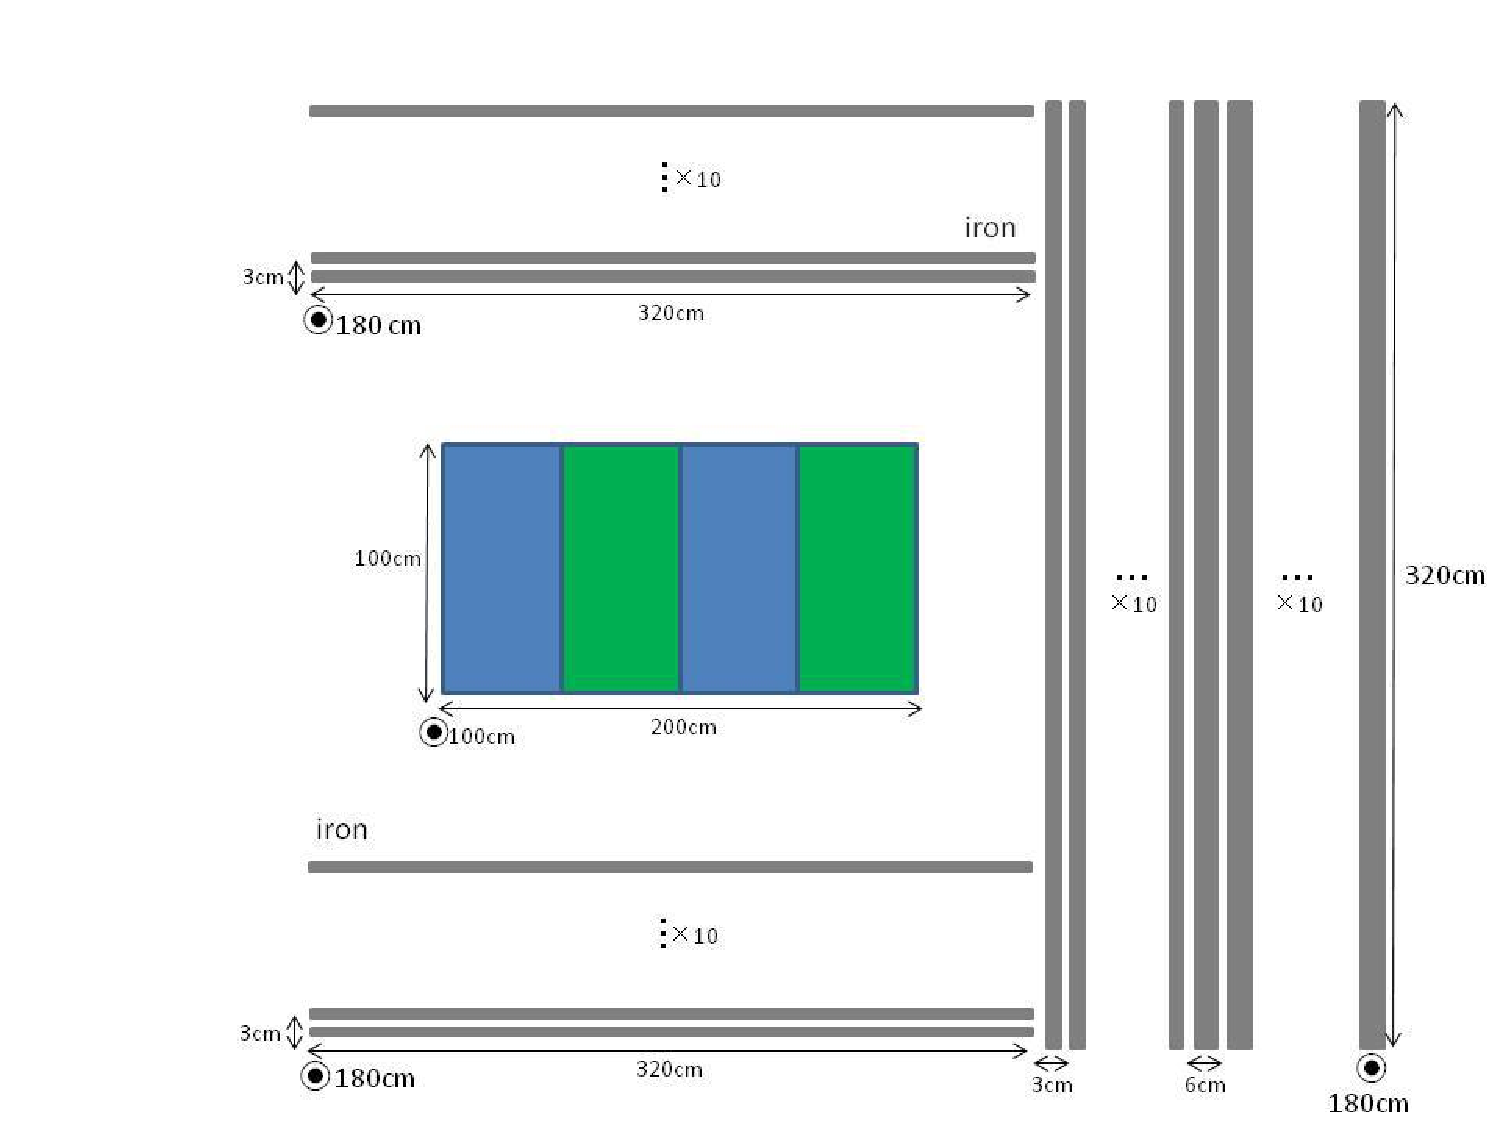
\includegraphics[width=0.8\linewidth]{fig/wagasci_mc_geometry.pdf}
% \includegraphics[width=0.8\linewidth]{fig/all_detector2.pdf}
\end{center}
\caption{
Geometry of the detectors in the Monte Carlo simulation.}
\label{fig:wagasci_mc_geometry}
\end{figure}

\begin{figure}[tbh]
\begin{center}
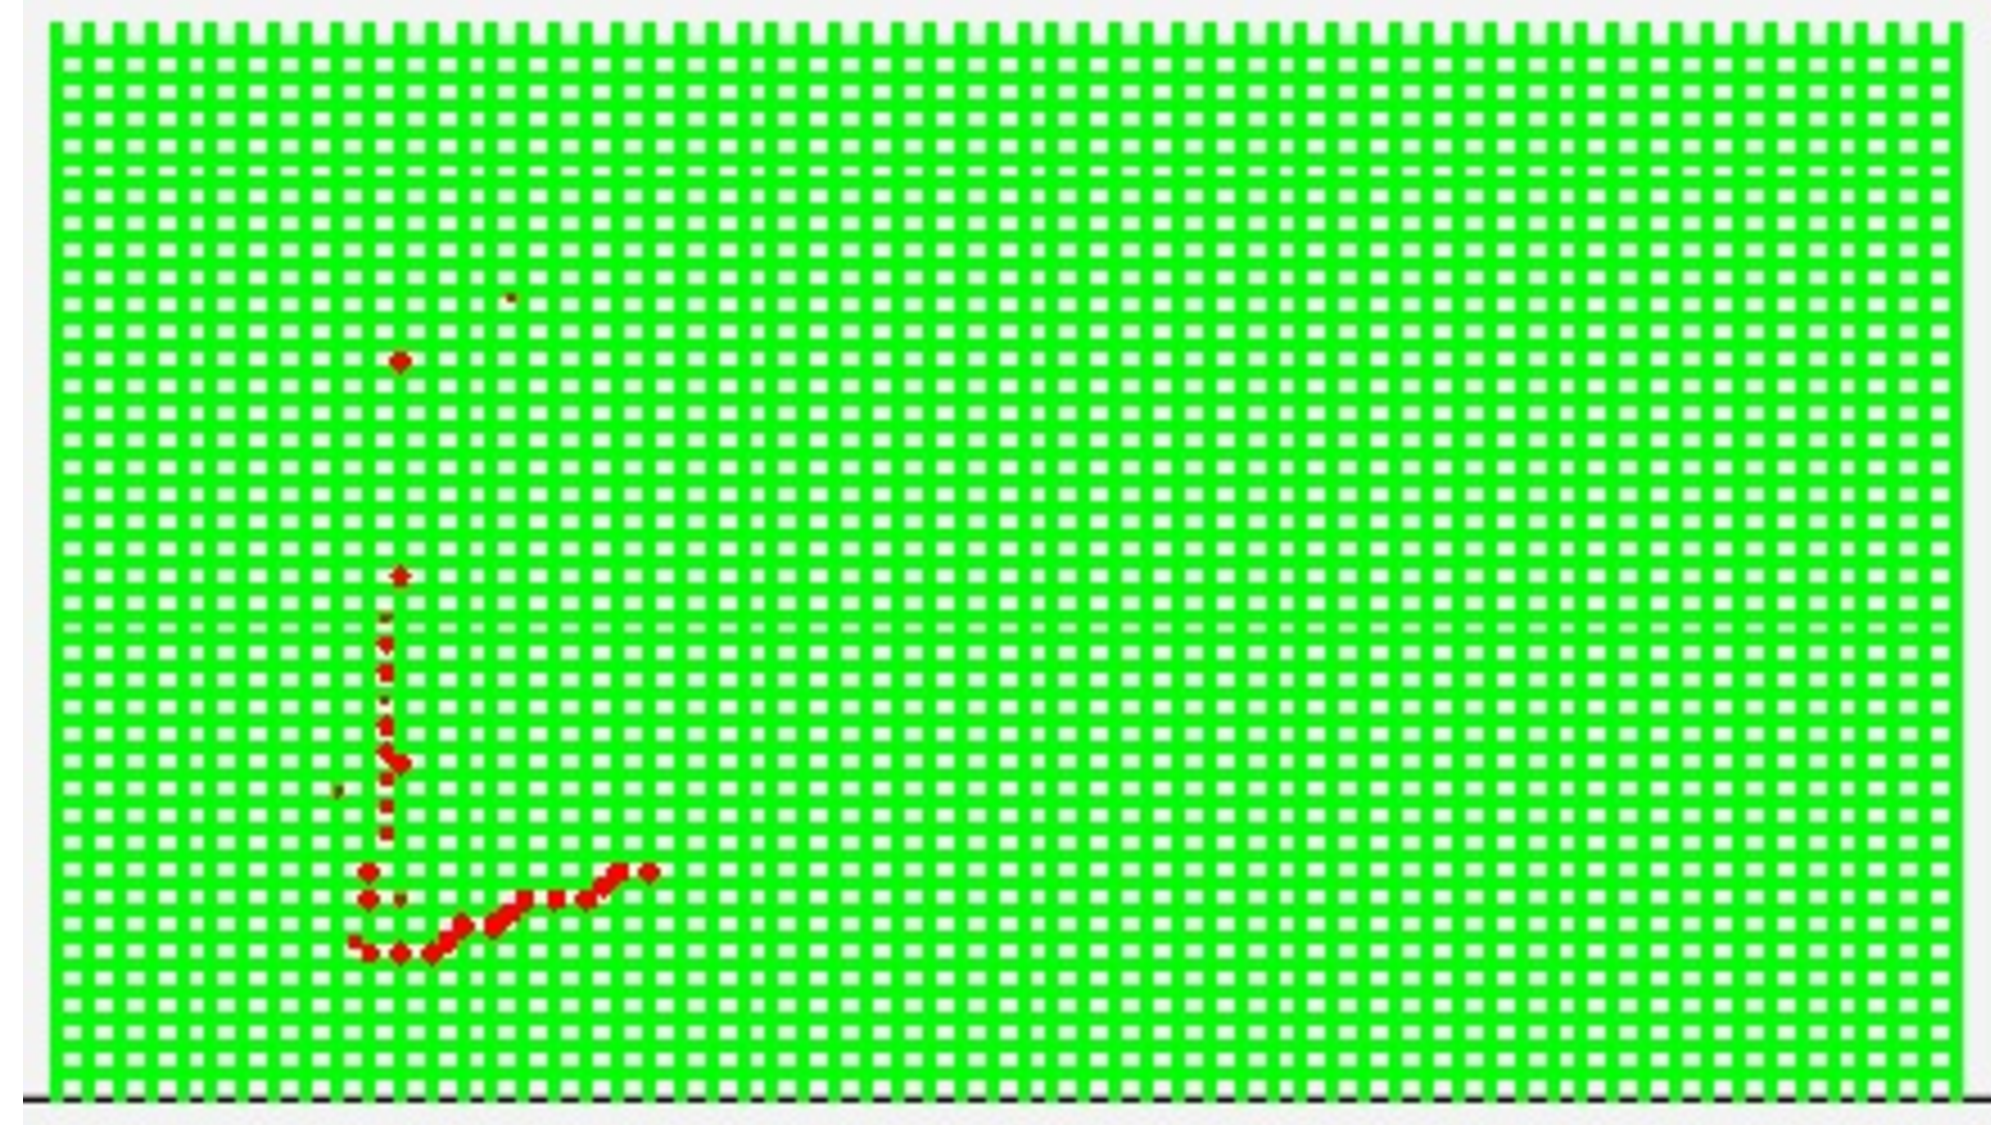
\includegraphics[width=0.8\linewidth]{fig/wagasci_event_display.pdf}
% \includegraphics[width=0.8\linewidth]{fig/all_detector2.pdf}
\end{center}
\caption{
An event display of MC event in WAGASCI detectors. Green lines are scintillators and red circles are the hit channels.}
\label{fig:wagasci_mc_geometry}
\end{figure}

In order to estimate backgrounds from neutrino interactions in the wall and floor of the experimental hall, the geometry of the experimental hall is implemented in the GEANT4-based detector simulation.


\subsubsection{Response of detector components}
The energy deposit inside the scintillator is converted into the number of photons. 
The effects of collection and attenuation of the light in the scintillator and the WLS fiber are simulated, and the MPPC response is also taken into account. 
The light yield is smeared according to statistical fluctuations and electrical noise.


\subsection{Track reconstruction}
To select neutrino interaction from the hit patterns, a track reconstruction algorithm is developed.
The flow of the track reconstruction is as follows.
\begin{enumerate}
\item Two-dimensional track reconstruction in each sub-detectors
\item Track matching among the sub-detectors
\item Three -dimensional track reconstruction
\end{enumerate}

Add explanation about two-dim reco, track matching and three-dim reco here.


\subsection{Event selection}

\subsubsection{Vertexing}


\subsubsection{Short track search}


\subsubsection{Fiducial volume cut}
The events with the track which starts in 5 cm from the wall of the WAGASCI module are rejected to remove the background from the outside as shown in Fig. \ref{fig:fv_cut}.

\begin{figure}[tbh]
  \begin{center}
   \begin{subfigure}{0.48\textwidth}
     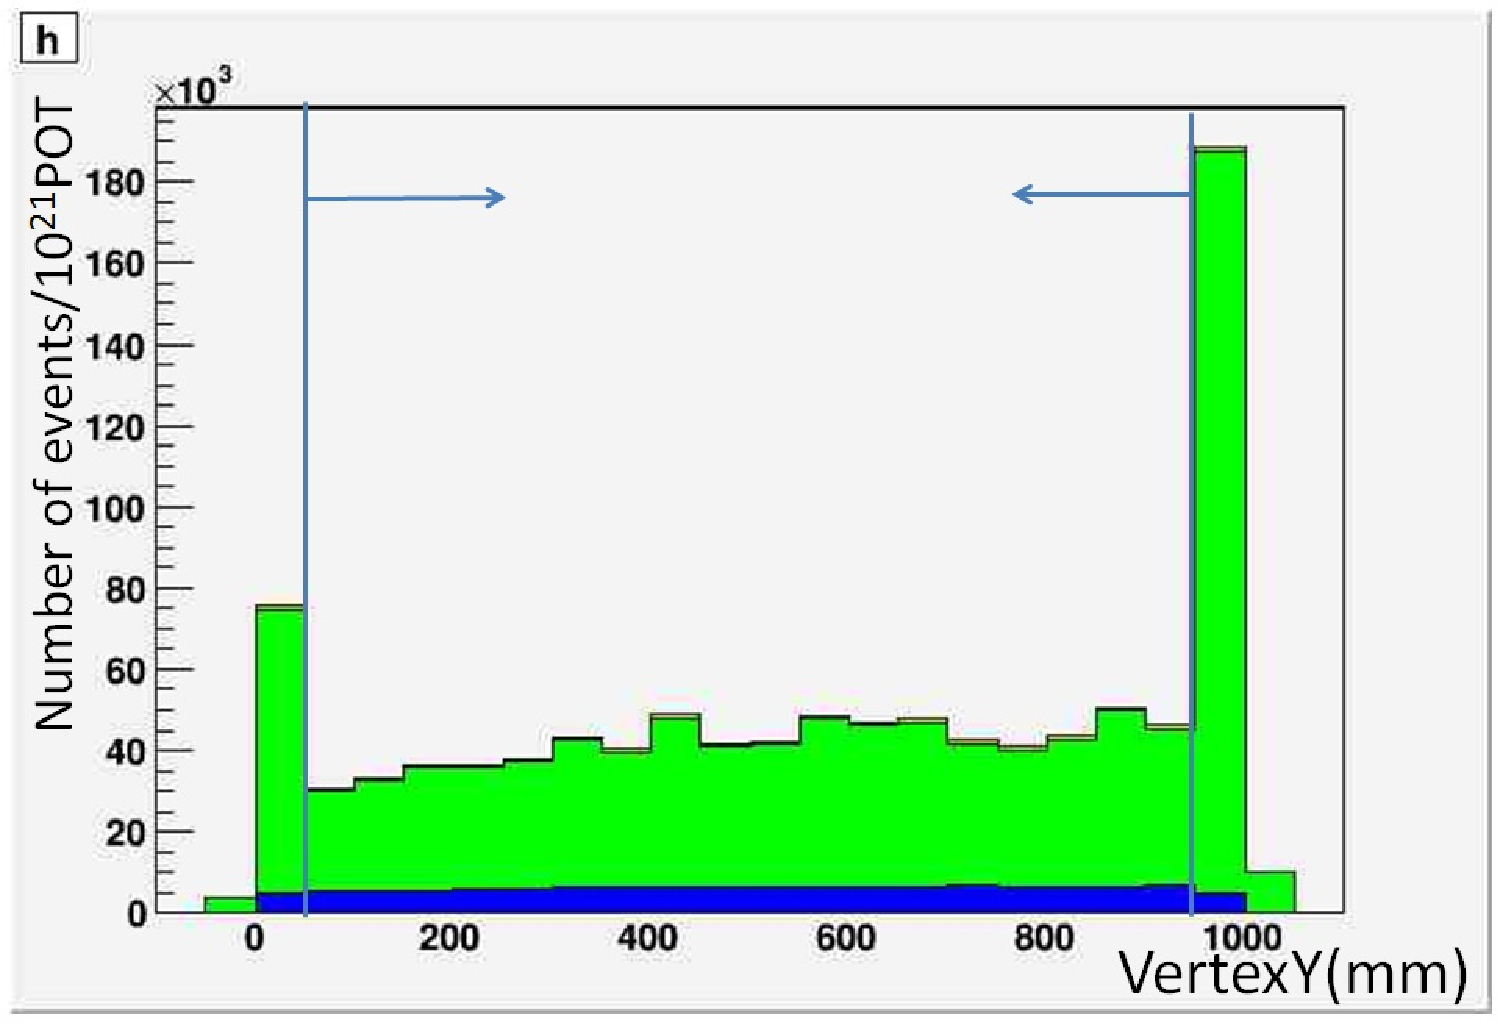
\includegraphics[width=\linewidth]{fig/fv_cut_y.pdf}
    \end{subfigure}
  \begin{subfigure}{0.48\textwidth}
      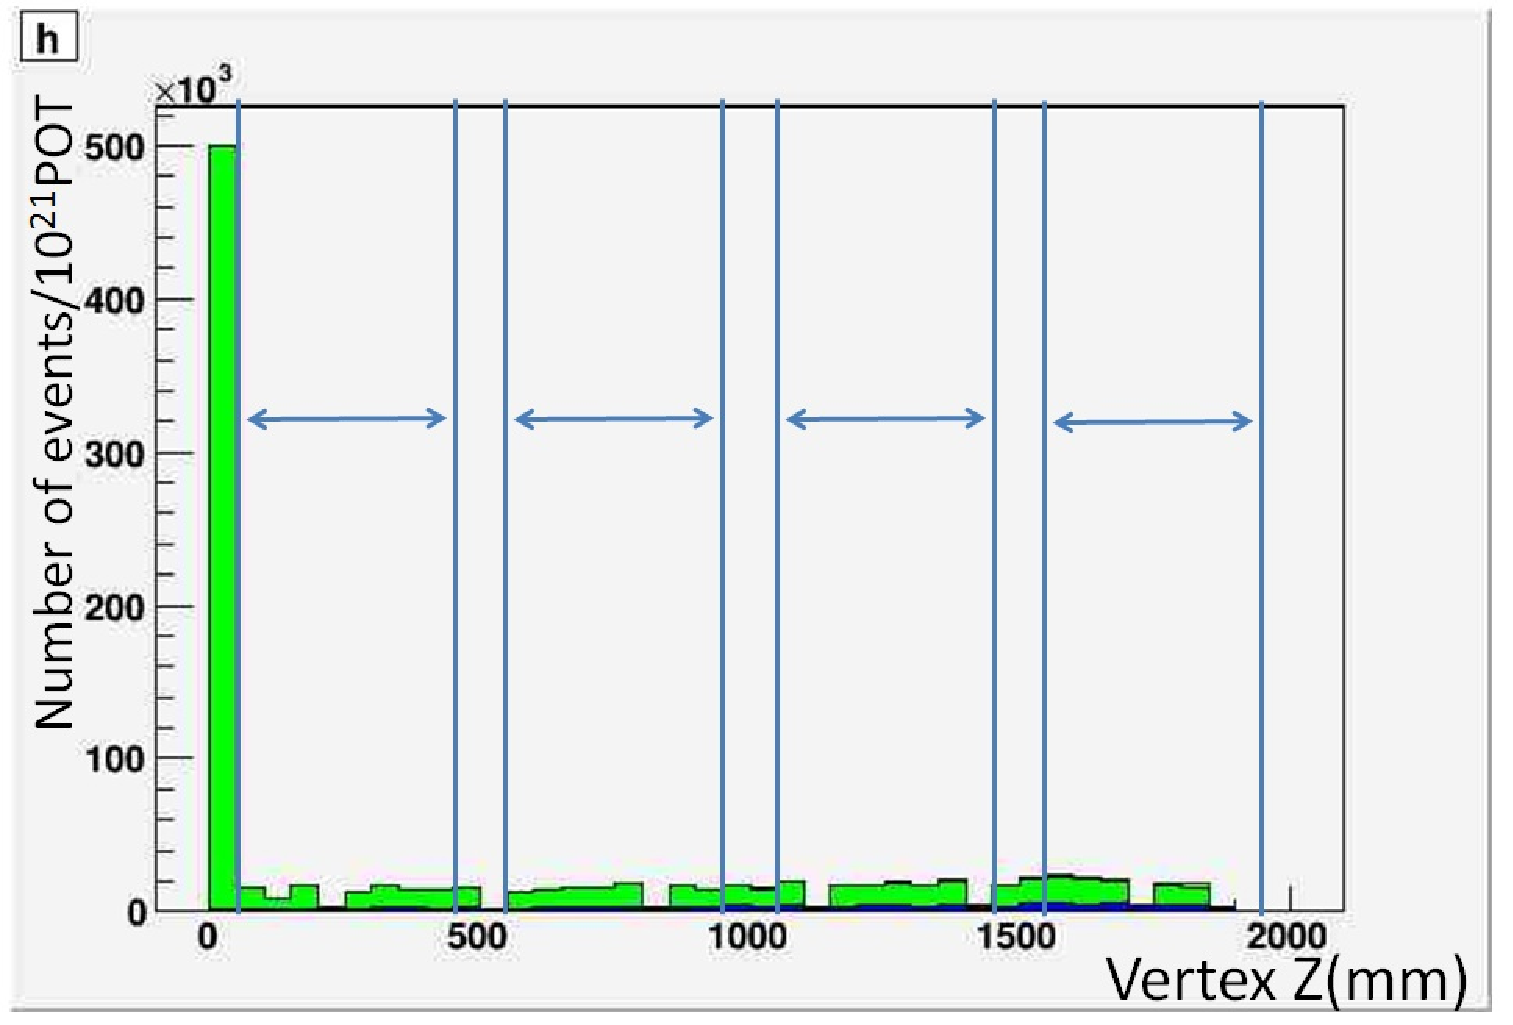
\includegraphics[width=\linewidth]{fig/fv_cut_z.pdf}
    \end{subfigure}    
    \end{center}
  \caption{Event selection with the vertex of the track.
Blue hist. are events from the WAGASCI modules, green hist. are events from the experimental hall, and yellow hist. are events from the Side-MRD modules and the downstream-MRD.
}
\label{fig:fv_cut}
\end{figure}


\subsubsection{Penetrated iron plates cut}


\begin{figure}[tbh]
  \begin{center}
   \begin{subfigure}{0.48\textwidth}
     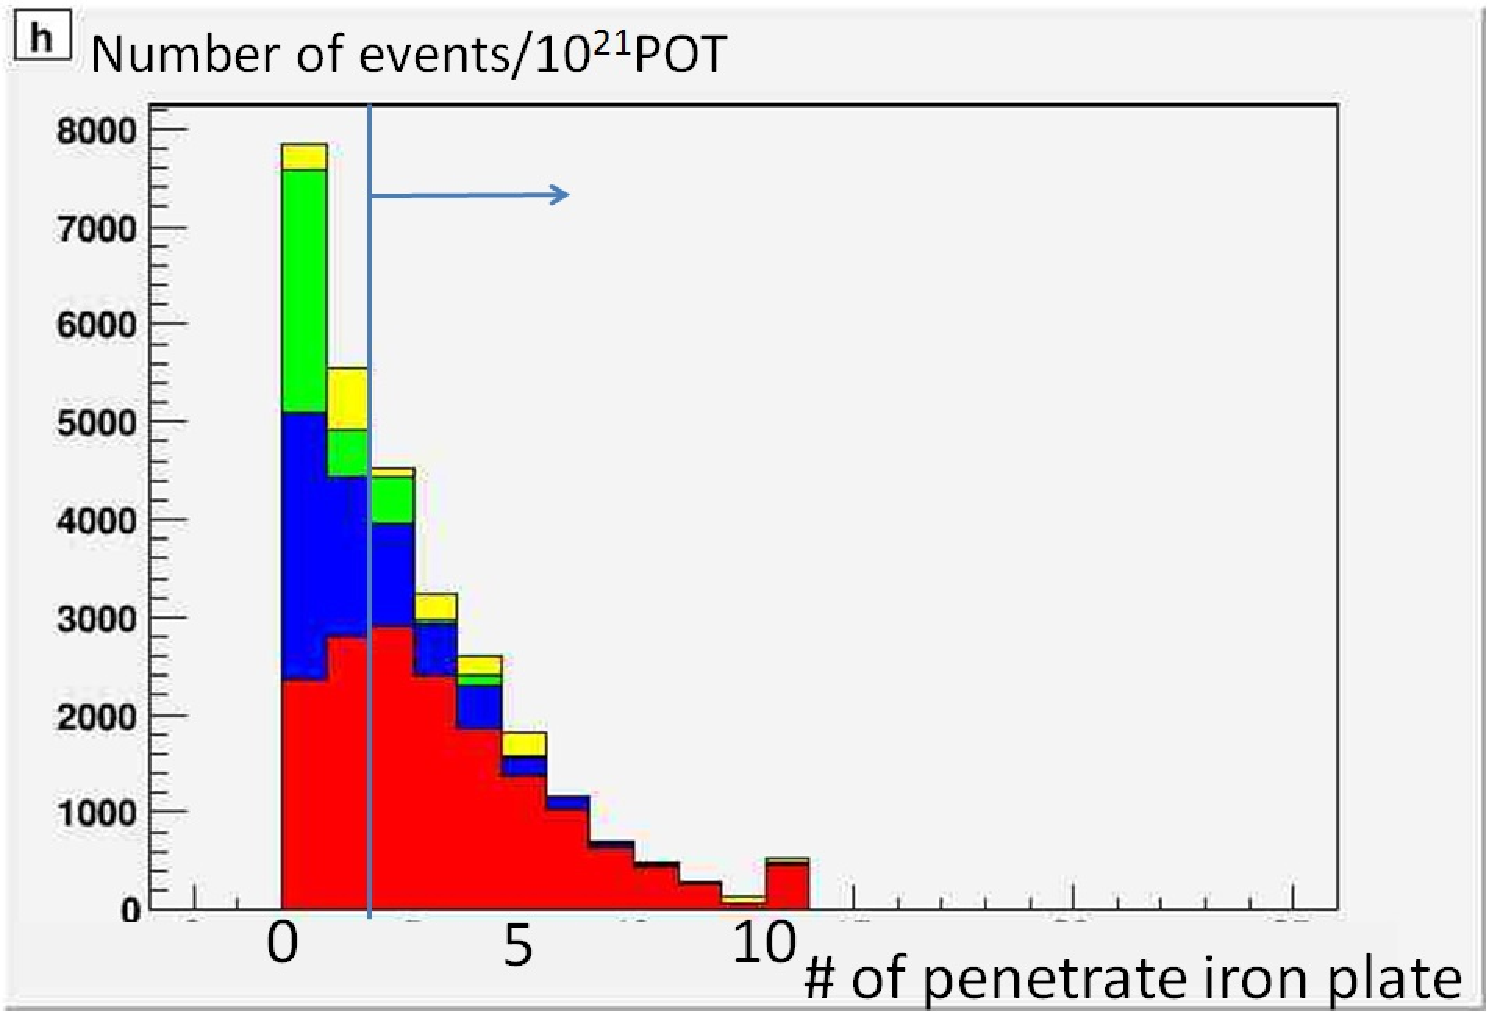
\includegraphics[width=\linewidth]{fig/penetrated_iron_plates_cut_sidemrd.pdf}
    \end{subfigure}
  \begin{subfigure}{0.48\textwidth}
      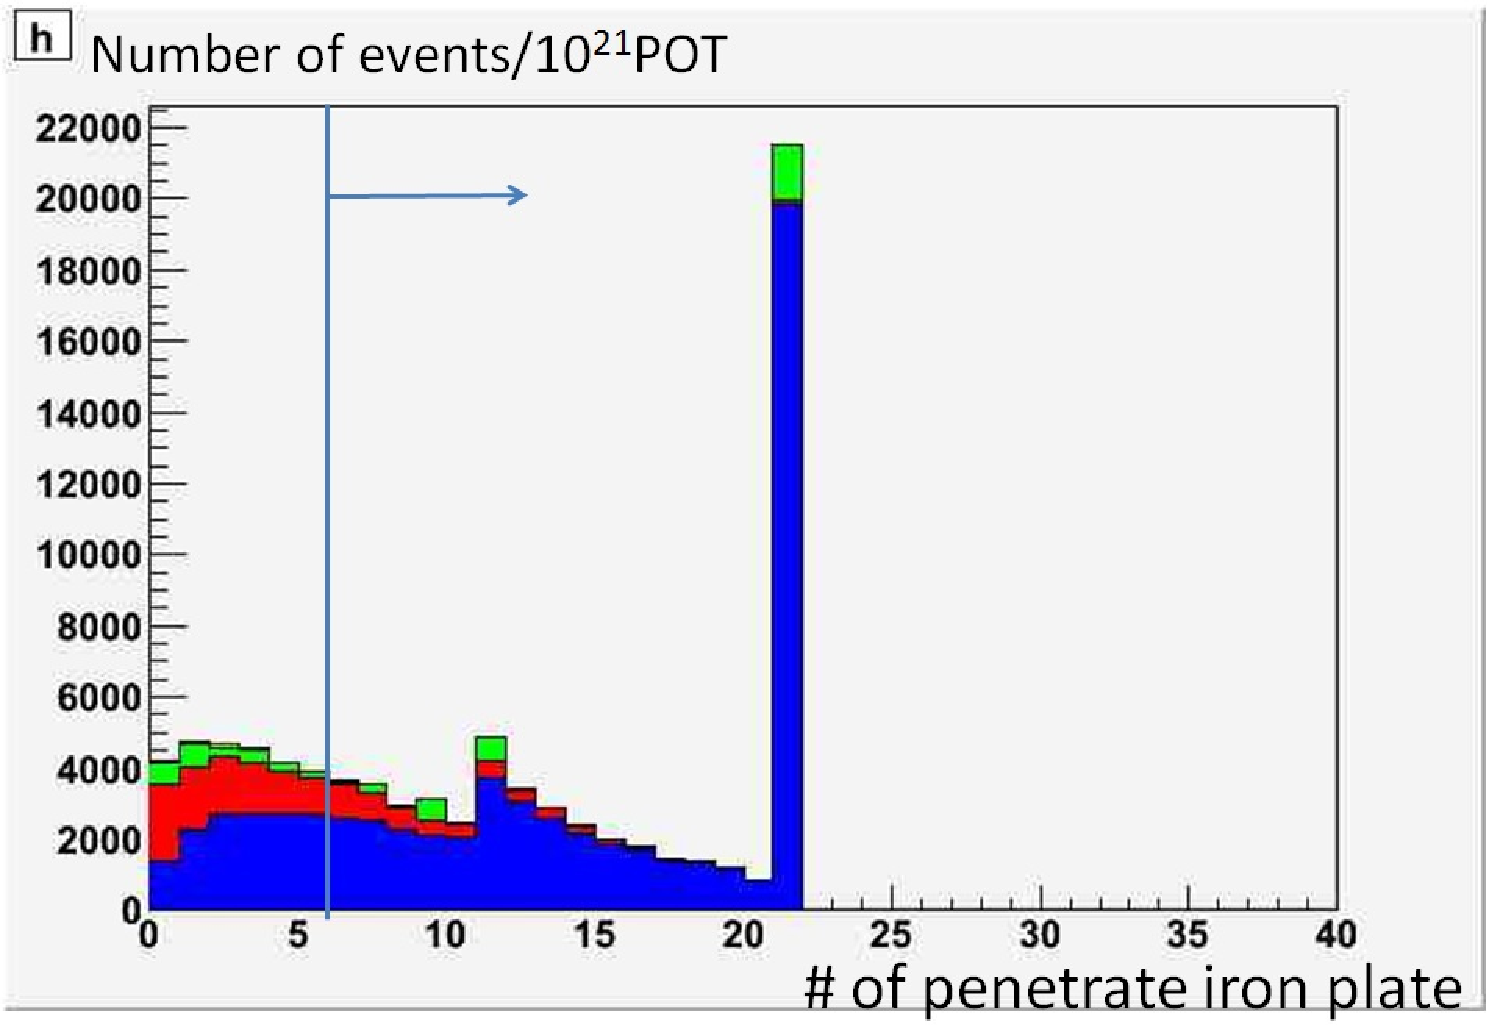
\includegraphics[width=\linewidth]{fig/penetrated_iron_plates_cut_babymind.pdf}
    \end{subfigure}    
    \end{center}
  \caption{
Event selection with the number of the penetrated iron plates in the Side-MRD modules (left) and the Baby-MIIND (right).
Blue and red hist. are events from the WAGASCI modules, green hist. are events from the experimental hall, and yellow hist. are events from the Side-MRD modules and the Baby-MIND.
}
\label{fig:penetrated_iron_plates_cut}
\end{figure}






